%%%%%%%%%%%%%%%%%%%%%%%%%%%%%%%
%% PACKAGE IMPORTS
%%%%%%%%%%%%%%%%%%%%%%%%%%%%%%%
\usepackage[tmargin=2cm,rmargin=1in,lmargin=1in,margin=0.85in,bmargin=2cm,footskip=.2in]{geometry}
\usepackage{amsmath,amsfonts,amsthm,amssymb,mathtools}
\usepackage[varbb]{newpxmath}
\usepackage{xfrac}
\usepackage[makeroom]{cancel}
\usepackage{mathtools}
\usepackage{bookmark}
\usepackage{enumitem}
\usepackage{hyperref,theoremref}
\hypersetup{
  pdftitle={Assignment},
  colorlinks=true, linkcolor=doc!90,
  bookmarksnumbered=true,
  bookmarksopen=true
}
\usepackage[most,many,breakable]{tcolorbox} % <-- For all fancy boxes
\usepackage{xcolor}
\usepackage{varwidth}
\usepackage{etoolbox}
\usepackage{nameref}
\usepackage{multicol,array}
\usepackage{tikz-cd}
\usepackage{tikz-3dplot}
\usepackage[ruled,vlined,linesnumbered]{algorithm2e}
\usepackage{comment}
\usepackage{import}
\usepackage{xifthen}
\usepackage{pdfpages}
\usepackage{transparent}
\usepackage{graphicx}   % <-- for .png/.jpg images
\usepackage{pgfplots}
\pgfplotsset{compat=newest}
\usepgfplotslibrary{colormaps}
\usepgfplotslibrary{fillbetween}

%%%%%%%%%%%%%%%%%%%%%%%%%%%%%%
% CUSTOM COMMENT STYLE FOR ALGORITHM2E
%%%%%%%%%%%%%%%%%%%%%%%%%%%%%%
\newcommand\mycommfont[1]{\footnotesize\ttfamily\textcolor{blue}{#1}}
\SetCommentSty{mycommfont}

%%%%%%%%%%%%%%%%%%%%%%%%%%%%%%
% COMMAND FOR FIGURES (SVG + PDF)
%%%%%%%%%%%%%%%%%%%%%%%%%%%%%%
\newcommand{\incfig}[1]{%
    \def\svgwidth{\columnwidth}
    \import{./figures/}{#1.pdf_tex}
}

%%%%%%%%%%%%%%%%%%%%%%%%%%%%%%
% CUSTOM QED SYMBOL (example)
%%%%%%%%%%%%%%%%%%%%%%%%%%%%%%
\usepackage{tikzsymbols}
\renewcommand\qedsymbol{$\Laughey$}

%%%%%%%%%%%%%%%%%%%%%%%%%%%%%%
% SELF MADE COLORS
%%%%%%%%%%%%%%%%%%%%%%%%%%%%%%
\definecolor{myg}{RGB}{56, 140, 70}
\definecolor{myb}{RGB}{45, 111, 177}
\definecolor{myr}{RGB}{199, 68, 64}
\definecolor{mytheorembg}{HTML}{F2F2F9}
\definecolor{mytheoremfr}{HTML}{00007B}
\definecolor{mylenmabg}{HTML}{FFFAF8}
\definecolor{mylenmafr}{HTML}{983b0f}
\definecolor{mypropbg}{HTML}{f2fbfc}
\definecolor{mypropfr}{HTML}{191971}
\definecolor{myexamplebg}{HTML}{F2FBF8}
\definecolor{myexamplefr}{HTML}{88D6D1}
\definecolor{myexampleti}{HTML}{2A7F7F}
\definecolor{mydefinitbg}{HTML}{E5E5FF}
\definecolor{mydefinitfr}{HTML}{3F3FA3}
\definecolor{notesgreen}{RGB}{0,162,0}
\definecolor{myp}{RGB}{197, 92, 212}
\definecolor{mygr}{HTML}{2C3338}
\definecolor{myred}{RGB}{127,0,0}
\definecolor{myyellow}{RGB}{169,121,69}
\definecolor{myexercisebg}{HTML}{F2FBF8}
\definecolor{myexercisefg}{HTML}{88D6D1}
\definecolor{pastelpink}{HTML}{FFE3ED} % For question & note envs
\definecolor{pastelFDF7C3}{HTML}{FDF7C3}

%%%%%%%%%%%%%%%%%%%%%%%%%%%%
% TCOLORBOX SETUPS FOR THEOREM-LIKE ENVIRONMENTS
%%%%%%%%%%%%%%%%%%%%%%%%%%%%

\setlength{\parindent}{1cm}

%================================
% THEOREM
%================================
\tcbuselibrary{theorems,skins,hooks}
\newtcbtheorem[no counter]{Theorem}{Theorem}
{%
  enhanced,
  breakable,
  colback = mytheorembg,
  frame hidden,
  boxrule = 0sp,
  borderline west = {2pt}{0pt}{mytheoremfr},
  sharp corners,
  detach title,
  before upper = \tcbtitle\par\smallskip,
  coltitle = mytheoremfr,
  fonttitle = \bfseries\sffamily,
  description font = \mdseries,
  separator sign none,
  segmentation style={solid, mytheoremfr},
}{th}

% Chapter-based if desired:
\newtcbtheorem[no counter]{theorem}{Theorem}
{%
  enhanced,
  breakable,
  colback = mytheorembg,
  frame hidden,
  boxrule = 0sp,
  borderline west = {2pt}{0pt}{mytheoremfr},
  sharp corners,
  detach title,
  before upper = \tcbtitle\par\smallskip,
  coltitle = mytheoremfr,
  fonttitle = \bfseries\sffamily,
  description font = \mdseries,
  separator sign none,
  segmentation style={solid, mytheoremfr},
}{th}

% Theorem "continuation" type box
\newtcolorbox{Theoremcon}
{%
  enhanced,
  breakable,
  colback = mytheorembg,
  frame hidden,
  boxrule = 0sp,
  borderline west = {2pt}{0pt}{mytheoremfr},
  sharp corners,
  description font = \mdseries,
  separator sign none
}

%================================
% COROLLARY
%================================
\newtcbtheorem[no counter]{Corollary}{Corollary}
{%
  enhanced,
  breakable,
  colback = myp!10,
  frame hidden,
  boxrule = 0sp,
  borderline west = {2pt}{0pt}{myp!85!black},
  sharp corners,
  detach title,
  before upper = \tcbtitle\par\smallskip,
  coltitle = myp!85!black,
  fonttitle = \bfseries\sffamily,
  description font = \mdseries,
  separator sign none,
  segmentation style={solid, myp!85!black},
}{th}

\newtcbtheorem[no counter]{corollary}{Corollary}
{%
  enhanced,
  breakable,
  colback = myp!10,
  frame hidden,
  boxrule = 0sp,
  borderline west = {2pt}{0pt}{myp!85!black},
  sharp corners,
  detach title,
  before upper = \tcbtitle\par\smallskip,
  coltitle = myp!85!black,
  fonttitle = \bfseries\sffamily,
  description font = \mdseries,
  separator sign none,
  segmentation style={solid, myp!85!black},
}{th}

%================================
% LEMMA
%================================
\newtcbtheorem[no counter]{Lenma}{Lenma}
{%
  enhanced,
  breakable,
  colback = mylenmabg,
  frame hidden,
  boxrule = 0sp,
  borderline west = {2pt}{0pt}{mylenmafr},
  sharp corners,
  detach title,
  before upper = \tcbtitle\par\smallskip,
  coltitle = mylenmafr,
  fonttitle = \bfseries\sffamily,
  description font = \mdseries,
  separator sign none,
  segmentation style={solid, mylenmafr},
}{th}

\newtcbtheorem[no counter]{lenma}{Lenma}
{%
  enhanced,
  breakable,
  colback = mylenmabg,
  frame hidden,
  boxrule = 0sp,
  borderline west = {2pt}{0pt}{mylenmafr},
  sharp corners,
  detach title,
  before upper = \tcbtitle\par\smallskip,
  coltitle = mylenmafr,
  fonttitle = \bfseries\sffamily,
  description font = \mdseries,
  separator sign none,
  segmentation style={solid, mylenmafr},
}{th}

%================================
% PROPOSITION
%================================
\newtcbtheorem[no counter]{Prop}{Proposition}
{%
  enhanced,
  breakable,
  colback = mypropbg,
  frame hidden,
  boxrule = 0sp,
  borderline west = {2pt}{0pt}{mypropfr},
  sharp corners,
  detach title,
  before upper = \tcbtitle\par\smallskip,
  coltitle = mypropfr,
  fonttitle = \bfseries\sffamily,
  description font = \mdseries,
  separator sign none,
  segmentation style={solid, mypropfr},
}{th}

\newtcbtheorem[no counter]{prop}{Proposition}
{%
  enhanced,
  breakable,
  colback = mypropbg,
  frame hidden,
  boxrule = 0sp,
  borderline west = {2pt}{0pt}{mypropfr},
  sharp corners,
  detach title,
  before upper = \tcbtitle\par\smallskip,
  coltitle = mypropfr,
  fonttitle = \bfseries\sffamily,
  description font = \mdseries,
  separator sign none,
  segmentation style={solid, mypropfr},
}{th}

%================================
% CLAIM
%================================
\newtcbtheorem[no counter]{claim}{Claim}
{%
  enhanced,
  breakable,
  colback = myg!10,
  frame hidden,
  boxrule = 0sp,
  borderline west = {2pt}{0pt}{myg},
  sharp corners,
  detach title,
  before upper = \tcbtitle\par\smallskip,
  coltitle = myg!85!black,
  fonttitle = \bfseries\sffamily,
  description font = \mdseries,
  separator sign none,
  segmentation style={solid, myg!85!black},
}{th}

%================================
% EXERCISE
%================================
\newtcbtheorem[no counter]{Exercise}{Exercise}
{%
  enhanced,
  breakable,
  colback = myexercisebg,
  frame hidden,
  boxrule = 0sp,
  borderline west = {2pt}{0pt}{myexercisefg},
  sharp corners,
  detach title,
  before upper = \tcbtitle\par\smallskip,
  coltitle = myexercisefg,
  fonttitle = \bfseries\sffamily,
  description font = \mdseries,
  separator sign none,
  segmentation style={solid, myexercisefg},
}{th}

\newtcbtheorem[no counter]{exercise}{Exercise}
{%
  enhanced,
  breakable,
  colback = myexercisebg,
  frame hidden,
  boxrule = 0sp,
  borderline west = {2pt}{0pt}{myexercisefg},
  sharp corners,
  detach title,
  before upper = \tcbtitle\par\smallskip,
  coltitle = myexercisefg,
  fonttitle = \bfseries\sffamily,
  description font = \mdseries,
  separator sign none,
  segmentation style={solid, myexercisefg},
}{th}

%================================
% EXAMPLE BOX
%================================
\definecolor{pastelExampleBg}{HTML}{70AF85}
\definecolor{greenPast}{HTML}{86C8BC}
\colorlet{myexamplebg}{pastelExampleBg!25!white}
\colorlet{myexamplefr}{pastelExampleBg!85!white}
\colorlet{myexampleti}{greenPast!40!black}

\newtcbtheorem[no counter]{Example}{Example}
{%
  colback = myexamplebg,
  breakable,
  colframe = myexamplefr,
  coltitle = myexampleti,
  boxrule = 1pt,
  sharp corners,
  detach title,
  before upper=\tcbtitle\par\smallskip,
  fonttitle = \bfseries,
  description font = \mdseries,
  separator sign none,
  description delimiters parenthesis
}{ex}

\newtcbtheorem[no counter]{example}{Example}
{%
  colback = myexamplebg,
  breakable,
  colframe = myexamplefr,
  coltitle = myexampleti,
  boxrule = 1pt,
  sharp corners,
  detach title,
  before upper=\tcbtitle\par\smallskip,
  fonttitle = \bfseries,
  description font = \mdseries,
  separator sign none,
  description delimiters parenthesis
}{ex}

% Example with a small image (rose):
\newtcbtheorem[no counter]{ExampleWithRose}{Example}
{%
  colback=myexamplebg,
  colframe=myexamplefr,
  coltitle=myexampleti,
  boxrule=1pt,
  sharp corners,
  enhanced,
  overlay={
    \node[anchor=south east] at (frame.south east) {
\includegraphics[width=1.5cm]{flow.png}};
  },
  detach title,
  before upper=\tcbtitle\par\smallskip,
  fonttitle=\bfseries,
  description font=\mdseries,
  separator sign none,
  description delimiters parenthesis
}{ex}

%================================
% DEFINITION BOX
%================================
\makeatletter
\definecolor{customblue}{RGB}{198, 220, 228}
\definecolor{darkblue}{RGB}{90, 120, 140}

\newtcbtheorem[no counter]{Definition}{Definition}{enhanced,
  before skip=2mm,after skip=2mm,
  colback=customblue!20, colframe=customblue!80,
  boxrule=0.5mm,
  attach boxed title to top left={xshift=1cm,yshift*=1mm-\tcboxedtitleheight},
  varwidth boxed title*=-3cm,
  boxed title style={
    frame code={
      \path[fill=customblue]
      ([yshift=-1mm,xshift=-1mm]frame.north west)
      arc[start angle=0,end angle=180,radius=1mm]
      ([yshift=-1mm,xshift=1mm]frame.north east)
      arc[start angle=180,end angle=0,radius=1mm];
      \path[left color=customblue,right color=customblue,
        middle color=customblue!90]
      ([xshift=-2mm]frame.north west) -- ([xshift=2mm]frame.north east)
      [rounded corners=1mm]-- ([xshift=1mm,yshift=-1mm]frame.north east)
      -- (frame.south east) -- (frame.south west)
      -- ([xshift=-1mm,yshift=-1mm]frame.north west)
      [sharp corners]-- cycle;
    },
    interior engine=empty,
  },
  fonttitle=\bfseries\color{darkblue},
  coltitle=darkblue,
  colbacktitle=customblue!80,
  title={#2}
}{def}

\newtcbtheorem[no counter]{definition}{Definition}{enhanced,
  before skip=2mm,after skip=2mm,
  colback=customblue!20, colframe=customblue!80,
  boxrule=0.5mm,
  attach boxed title to top left={xshift=1cm,yshift*=1mm-\tcboxedtitleheight},
  varwidth boxed title*=-3cm,
  boxed title style={
    frame code={
      \path[fill=customblue]
      ([yshift=-1mm,xshift=-1mm]frame.north west)
      arc[start angle=0,end angle=180,radius=1mm]
      ([yshift=-1mm,xshift=1mm]frame.north east)
      arc[start angle=180,end angle=0,radius=1mm];
      \path[left color=customblue,right color=customblue,
        middle color=customblue!90]
      ([xshift=-2mm]frame.north west) -- ([xshift=2mm]frame.north east)
      [rounded corners=1mm]-- ([xshift=1mm,yshift=-1mm]frame.north east)
      -- (frame.south east) -- (frame.south west)
      -- ([xshift=-1mm,yshift=-1mm]frame.north west)
      [sharp corners]-- cycle;
    },
    interior engine=empty,
  },
  fonttitle=\bfseries\color{darkblue},
  coltitle=darkblue,
  colbacktitle=customblue!80,
  title={#2}
}{def}
\makeatother

% Definition with image in bottom-right corner
\makeatletter
\definecolor{customblue2}{RGB}{198, 234, 245}
\newtcbtheorem[no counter]{DefinitionWithImage}{Definition}{enhanced,
  before skip=2mm,
  after skip=2mm,
  colback=customblue2!40,
  colframe=customblue2!80!black,
  boxrule=0.5mm,
  attach boxed title to top left={xshift=1cm,yshift*=1mm-\tcboxedtitleheight},
  varwidth boxed title*=-3cm,
  boxed title style={
    frame code={
      \path[fill=customblue2]
      ([yshift=-1mm,xshift=-1mm]frame.north west)
      arc[start angle=0,end angle=180,radius=1mm]
      ([yshift=-1mm,xshift=1mm]frame.north east)
      arc[start angle=180,end angle=0,radius=1mm];
      \path[left color=customblue2,right color=customblue2,
        middle color=customblue2!90]
      ([xshift=-2mm]frame.north west) -- ([xshift=2mm]frame.north east)
      [rounded corners=1mm]-- ([xshift=1mm,yshift=-1mm]frame.north east)
      -- (frame.south east) -- (frame.south west)
      -- ([xshift=-1mm,yshift=-1mm]frame.north west)
      [sharp corners]-- cycle;
    },
    interior engine=empty,
  },
  fonttitle=\bfseries\color{darkblue},
  coltitle=darkblue,
  colbacktitle=customblue2!80,
  title={#2},
  overlay unbroken and last={
    \node[anchor=south east,xshift=-2mm,yshift=2mm] at (frame.south east) {
\includegraphics[width=1 cm]{slime.png}};
  }
}{def}
\makeatother

%================================
% SOLUTION BOX
%================================
\makeatletter
\newtcolorbox{solution}{enhanced,
  breakable,
  colback=white,
  colframe=myg!80!black,
  attach boxed title to top left={yshift*=-\tcboxedtitleheight},
  title=Solution,
  boxed title size=title,
  boxed title style={%
    sharp corners,
    rounded corners=northwest,
    colback=tcbcolframe,
    boxrule=0pt,
  },
  underlay boxed title={%
    \path[fill=tcbcolframe] (title.south west)--(title.south east)
    to[out=0, in=180] ([xshift=5mm]title.east)--
    (title.center-|frame.east)
    [rounded corners=\kvtcb@arc] |-
    (frame.north) -| cycle;
  },
}
\makeatother

%================================
% "Wrong Concept" BOX
%================================
\newtcbtheorem[no counter]{wconc}{Wrong Concept}{
  breakable,
  enhanced,
  colback=white,
  colframe=myr,
  arc=0pt,
  outer arc=0pt,
  fonttitle=\bfseries\sffamily\large,
  colbacktitle=myr,
  attach boxed title to top left={},
  boxed title style={
    enhanced,
    skin=enhancedfirst jigsaw,
    arc=3pt,
    bottom=0pt,
    interior style={fill=myr}
  }
}{def}

%================================
% NOTE BOX (Pastel Pink)
%================================
\usetikzlibrary{arrows,calc,shadows.blur}
\tcbuselibrary{skins}
\newtcolorbox{note}[1][]{%
  enhanced jigsaw,
  colback=pastelpink,
  colframe=pastelpink,
  size=small,
  boxrule=1pt,
  title=\textbf{Note:-},
  halign title=flush center,
  coltitle=black,
  breakable,
  drop shadow=black!50!white,
  attach boxed title to top left={xshift=1cm,yshift=-\tcboxedtitleheight/2,yshifttext=-\tcboxedtitleheight/2},
  minipage boxed title=1.5cm,
  boxed title style={%
    colback=white,
    size=fbox,
    boxrule=1pt,
    boxsep=2pt,
    underlay={%
      \coordinate (dotA) at ($(interior.west) + (-0.5pt,0)$);
      \coordinate (dotB) at ($(interior.east) + (0.5pt,0)$);
      \begin{scope}
        \clip (interior.north west) rectangle ([xshift=3ex]interior.east);
        \filldraw [white, blur shadow={shadow opacity=60, shadow yshift=-.75ex}, rounded corners=2pt] (interior.north west) rectangle (interior.south east);
      \end{scope}
      \begin{scope}[pastelpink]
        \fill (dotA) circle (2pt);
        \fill (dotB) circle (2pt);
      \end{scope}
    },
  },
  #1,
}

%================================
% NOTE BOX (Pastel Pink with Image)
%================================
\newtcolorbox{noteWithImage}[1][]{%
  enhanced jigsaw,
  colback=pastelFDF7C3!70!white,
  colframe=pastelFDF7C3!80!white,
  size=small,
  boxrule=1pt,
  title=\textbf{Note:-},
  halign title=flush center,
  coltitle=black,
  breakable,
  drop shadow=black!50!white,
  attach boxed title to top left={xshift=1cm,yshift=-\tcboxedtitleheight/2,yshifttext=-\tcboxedtitleheight/2},
  minipage boxed title=1.5cm,
  boxed title style={%
    colback=white,
    size=fbox,
    boxrule=1pt,
    boxsep=2pt,
    underlay={%
      \coordinate (dotA) at ($(interior.west) + (-0.5pt,0)$);
      \coordinate (dotB) at ($(interior.east) + (0.5pt,0)$);
      \begin{scope}
        \clip (interior.north west) rectangle ([xshift=3ex]interior.east);
        \filldraw [white, blur shadow={shadow opacity=60, shadow yshift=-.75ex}, rounded corners=2pt] (interior.north west) rectangle (interior.south east);
      \end{scope}
      \begin{scope}[pastelFDF7C3!80!white]
        \fill (dotA) circle (2pt);
        \fill (dotB) circle (2pt);
      \end{scope}
    },
  },
  overlay unbroken and last={
    \node[anchor=south east,xshift=-2mm,yshift=1mm] at (frame.south east) {
\includegraphics[width=1cm]{lot.png}};
  },
  #1,
}

%%%%%%%%%%%%%%%%%%%%%%%%%%%%%%
% QUESTION BOX (PASTEL PINK)
%%%%%%%%%%%%%%%%%%%%%%%%%%%%%%
\makeatletter
\newtcbtheorem[no counter]{question}{Question}{enhanced,
  breakable,
  colback=pastelpink!60,
  colframe=pastelpink!90!black,
  attach boxed title to top left={yshift*=-\tcboxedtitleheight},
  fonttitle=\bfseries,
  title={#2},
  boxed title size=title,
  boxed title style={%
    sharp corners,
    rounded corners=northwest,
    colback=tcbcolframe,
    boxrule=0pt,
  },
  underlay boxed title={%
    \path[fill=tcbcolframe] (title.south west)--(title.south east)
    to[out=0, in=180] ([xshift=5mm]title.east)--
    (title.center-|frame.east)
    [rounded corners=\kvtcb@arc] |-
    (frame.north) -| cycle;
  },
  #1
}{def}
\makeatother

%%%%%%%%%%%%%%%%%%%%%%%%%%%%%%
% SELF MADE COMMANDS
%%%%%%%%%%%%%%%%%%%%%%%%%%%%%%
\newcommand{\thm}[2]{\begin{Theorem}{#1}{}#2\end{Theorem}}
\newcommand{\cor}[2]{\begin{Corollary}{#1}{}#2\end{Corollary}}
\newcommand{\mlenma}[2]{\begin{Lenma}{#1}{}#2\end{Lenma}}
\newcommand{\mprop}[2]{\begin{Prop}{#1}{}#2\end{Prop}}
\newcommand{\clm}[3]{\begin{claim}{#1}{#2}#3\end{claim}}
\newcommand{\wc}[2]{\begin{wconc}{#1}{}\setlength{\parindent}{1cm}#2\end{wconc}}
\newcommand{\thmcon}[1]{\begin{Theoremcon}{#1}\end{Theoremcon}}
\newcommand{\exer}[2]{\begin{Exercise}{#1}{}#2\end{Exercise}}
\newcommand{\ex}[2]{\begin{Example}{#1}{}#2\end{Example}}
\newcommand{\dfn}[2]{\begin{Definition}[colbacktitle=red!75!black]{#1}{}#2\end{Definition}}
\newcommand{\dfnc}[2]{\begin{definition}[colbacktitle=red!75!black]{#1}{}#2\end{definition}}
\newcommand{\qs}[2]{\begin{question}{#1}{}#2\end{question}}
\newcommand{\pf}[2]{\begin{myproof}[#1]#2\end{myproof}}
\newcommand{\nt}[1]{\begin{note}#1\end{note}}
\newcommand{\insertpng}[2][1]{\begin{center} \includegraphics[scale=#1]{#2} \end{center}} 

\newcommand{\defrose}[2]{%
    \begin{DefinitionWithImage}{#1}%
        #2%
    \end{DefinitionWithImage}%
}
\newcommand{\exrose}[2]{%
    \begin{ExampleWithRose}{#1}%
        #2%
    \end{ExampleWithRose}%
}
\newcommand{\ntimg}[2][]{%
    \begin{noteWithImage}[#1]%
        #2%
    \end{noteWithImage}%
}

\newcommand*\circled[1]{\tikz[baseline=(char.base)]{
  \node[shape=circle,draw,inner sep=1pt] (char) {#1};}}
\newcommand\getcurrentref[1]{%
  \ifnumequal{\value{#1}}{0}{??}{\the\value{#1}}%
}
\newcommand{\getCurrentSectionNumber}{\getcurrentref{section}}
\newenvironment{myproof}[1][\proofname]{%
  \proof[\bfseries #1: ]%
}{\endproof}

\newcommand{\mclm}[2]{\begin{myclaim}[#1]#2\end{myclaim}}
\newenvironment{myclaim}[1][\claimname]{\proof[\bfseries #1: ]}{}

\newcounter{mylabelcounter}
\makeatletter
\newcommand{\setword}[2]{%
  \phantomsection
  #1\def\@currentlabel{\unexpanded{#1}}\label{#2}%
}
\makeatother

\tikzset{
  symbol/.style={
    draw=none,
    every to/.append style={
      edge node={node [sloped, allow upside down, auto=false]{$#1$}}
    }
  }
}

% Parentheses, absolute values, norms, etc.
\DeclarePairedDelimiter{\abs}{\lvert}{\rvert}
\DeclarePairedDelimiter{\norm}{\lVert}{\rVert}
\DeclarePairedDelimiter{\ceil}{\lceil}{\rceil}
\DeclarePairedDelimiter{\floor}{\lfloor}{\rfloor}
\DeclarePairedDelimiter{\round}{\lfloor}{\rceil}

% custom differential
\newsavebox\diffdbox
\newcommand{\slantedromand}{{\mathpalette\makesl{d}}}
\newcommand{\makesl}[2]{%
\begingroup
\sbox{\diffdbox}{$\mathsurround=0pt#1\mathrm{#2}$}%
\pdfsave
\pdfsetmatrix{1 0 0.2 1}%
\rlap{\usebox{\diffdbox}}%
\pdfrestore
\hskip\wd\diffdbox
\endgroup
}
\newcommand{\dd}[1][]{\ensuremath{\mathop{}\!\ifstrempty{#1}{%
\slantedromand\@ifnextchar^{\hspace{0.2ex}}{\hspace{0.1ex}}}%
{\slantedromand\hspace{0.2ex}^{#1}}}}
\providecommand{\dv}[3][]{\frac{\dd^{#1} #2}{\dd #3^{#1}}}
\providecommand*{\pdv}[3][]{\frac{\partial^{#1}#2}{\partial#3^{#1}}}

\DeclareMathOperator{\Lap}{\mathcal{L}}
\DeclareMathOperator{\Var}{Var}
\DeclareMathOperator{\Cov}{Cov}
\DeclareMathOperator{\E}{E}

%%%%%%%%%%%%%%%%%%%%%%%%%%%%%%%%%%%%%%%%%%%
% TABLE OF CONTENTS FANCY SETUP (OPTIONAL)
%%%%%%%%%%%%%%%%%%%%%%%%%%%%%%%%%%%%%%%%%%%
\usepackage{tikz}
\definecolor{doc}{HTML}{AD6989}
\usepackage{titletoc}
\contentsmargin{0cm}
\titlecontents{chapter}[3.7pc]
{\addvspace{30pt}%
 \begin{tikzpicture}[remember picture, overlay]%
  \draw[fill=doc!60,draw=doc!60] (-7,-.1) rectangle (-0.9,.5);%
  \pgftext[left,x=-3.5cm,y=0.2cm]{\color{white}\Large\sc\bfseries Chapter\ \thecontentslabel};%
 \end{tikzpicture}\color{doc!60}\large\sc\bfseries}%
{}
{}
{\;\titlerule\;\large\sc\bfseries Page \thecontentspage
 \begin{tikzpicture}[remember picture, overlay]
  \draw[fill=doc!60,draw=doc!60] (2pt,0) rectangle (4,0.1pt);
 \end{tikzpicture}}%
\titlecontents{section}[3.7pc]
{\addvspace{2pt}}
{\contentslabel[\thecontentslabel]{2pc}}
{}
{\hfill\small \thecontentspage}
[]
\titlecontents*{subsection}[3.7pc]
{\addvspace{-1pt}\small}
{}
{}
{\ --- \small\thecontentspage}
[ \textbullet\ ][]
\makeatletter
\renewcommand{\tableofcontents}{%
  \chapter*{%
   \vspace*{-20\p@}%
   \begin{tikzpicture}[remember picture, overlay]%
    \pgftext[right,x=15cm,y=0.2cm]{\color{doc!60}\Huge\sc\bfseries \contentsname};%
    \draw[fill=doc!60,draw=doc!60] (13,-.75) rectangle (20,1);%
    \clip (13,-.75) rectangle (20,1);
    \pgftext[right,x=15cm,y=0.2cm]{\color{white}\Huge\sc\bfseries \contentsname};%
   \end{tikzpicture}}%
  \@starttoc{toc}}
\makeatother

%%%%%%%%%%%%%%%%%%%%%%%%%%%%%%%%%%%%%%%%%%%%%%%%%%%%%%%%%%%%%%%%%%%%
%% NEW PASTEL BOXES: REMARK, AXIOM, FACT, CONJECTURE, OBSERVATION,
%% KEY IDEA, PROOF SKETCH, BASE CASE, INDUCTIVE STEP
%%%%%%%%%%%%%%%%%%%%%%%%%%%%%%%%%%%%%%%%%%%%%%%%%%%%%%%%%%%%%%%%%%%%

%% REMARK
\definecolor{myremarkbg}{HTML}{EEE8FD}  % Very light lavender
\definecolor{myremarkfr}{HTML}{7955D3}  % Deeper lavender/purple
\newtcbtheorem[no counter]{Remark}{Remark}
{%
  enhanced,
  breakable,
  colback = myremarkbg,
  frame hidden,
  boxrule = 0pt,
  borderline west = {2pt}{0pt}{myremarkfr},
  sharp corners,
  detach title,
  before upper = \tcbtitle\par\smallskip,
  coltitle = myremarkfr,
  fonttitle = \bfseries\sffamily,
  description font = \mdseries,
  separator sign none,
  segmentation style={solid, myremarkfr},
}{rm}

%% AXIOM
\definecolor{myaxiombg}{HTML}{FFF9E6}  % Pastel yellow
\definecolor{myaxiomfr}{HTML}{D7A123}  % Deeper golden
\newtcbtheorem[no counter]{Axiom}{Axiom}
{%
  enhanced,
  breakable,
  colback = myaxiombg,
  frame hidden,
  boxrule = 0pt,
  borderline west = {2pt}{0pt}{myaxiomfr},
  sharp corners,
  detach title,
  before upper = \tcbtitle\par\smallskip,
  coltitle = myaxiomfr,
  fonttitle = \bfseries\sffamily,
  description font = \mdseries,
  separator sign none,
  segmentation style={solid, myaxiomfr},
}{ax}

%% FACT
\definecolor{myfactbg}{HTML}{F2FBE5}  % Pale green
\definecolor{myfactfr}{HTML}{679436}  % Medium green
\newtcbtheorem[no counter]{Fact}{Fact}
{%
  enhanced,
  breakable,
  colback = myfactbg,
  frame hidden,
  boxrule = 0pt,
  borderline west = {2pt}{0pt}{myfactfr},
  sharp corners,
  detach title,
  before upper = \tcbtitle\par\smallskip,
  coltitle = myfactfr,
  fonttitle = \bfseries\sffamily,
  description font = \mdseries,
  separator sign none,
  segmentation style={solid, myfactfr},
}{fc}

%% CONJECTURE
\definecolor{myconjbg}{HTML}{F5EEFC}  % Light pastel purple/pink
\definecolor{myconjfr}{HTML}{6A0DAD}  % Deep purple
\newtcbtheorem[no counter]{Conjecture}{Conjecture}
{%
  enhanced,
  breakable,
  colback = myconjbg,
  frame hidden,
  boxrule = 0pt,
  borderline west = {2pt}{0pt}{myconjfr},
  sharp corners,
  detach title,
  before upper = \tcbtitle\par\smallskip,
  coltitle = myconjfr,
  fonttitle = \bfseries\sffamily,
  description font = \mdseries,
  separator sign none,
  segmentation style={solid, myconjfr},
}{cj}

%% OBSERVATION
\definecolor{myobsbg}{HTML}{FFF8D4}  % Very light pastel yellow
\definecolor{myobsfr}{HTML}{E1C16A}  % Slightly darker golden
\newtcbtheorem[no counter]{Observation}{Observation}
{%
  enhanced,
  breakable,
  colback = myobsbg,
  frame hidden,
  boxrule = 0pt,
  borderline west = {2pt}{0pt}{myobsfr},
  sharp corners,
  detach title,
  before upper = \tcbtitle\par\smallskip,
  coltitle = myobsfr,
  fonttitle = \bfseries\sffamily,
  description font = \mdseries,
  separator sign none,
  segmentation style={solid, myobsfr},
}{obs}

%% KEY IDEA (un-numbered)
\definecolor{myideabg}{HTML}{E7F2FA}
\definecolor{myideafr}{HTML}{174D8C}
\newtcolorbox{keyidea}{
  enhanced,
  breakable,
  colback = myideabg,
  frame hidden,
  boxrule = 0pt,
  borderline west = {2pt}{0pt}{myideafr},
  sharp corners,
  title = {\bfseries Key Idea},
  detach title,
  before upper = \tcbtitle\par\smallskip,
  coltitle = myideafr,
}

%% PROOF SKETCH (un-numbered)
\definecolor{myoutlinebg}{HTML}{EBF8FF}
\definecolor{myoutlinefr}{HTML}{3B7EA1}
\newtcolorbox{proofsketch}{
  enhanced,
  breakable,
  colback = myoutlinebg,
  frame hidden,
  boxrule = 0pt,
  borderline west = {2pt}{0pt}{myoutlinefr},
  sharp corners,
  title = {\bfseries Proof Sketch},
  detach title,
  before upper = \tcbtitle\par\smallskip,
  coltitle = myoutlinefr,
}

%% BASE CASE (un-numbered)
\definecolor{mybasebg}{HTML}{F2FBF8}
\definecolor{mybasefr}{HTML}{88D6D1}
\newtcolorbox{basecase}{
  enhanced,
  breakable,
  colback = mybasebg,
  frame hidden,
  boxrule = 0pt,
  borderline west = {2pt}{0pt}{mybasefr},
  sharp corners,
  title = {\bfseries Base Case},
  detach title,
  before upper = \tcbtitle\par\smallskip,
  coltitle = mybasefr,
}

%% INDUCTIVE STEP (un-numbered)
\newtcolorbox{inductstep}{
  enhanced,
  breakable,
  colback = mybasebg,
  frame hidden,
  boxrule = 0pt,
  borderline west = {2pt}{0pt}{mybasefr},
  sharp corners,
  title = {\bfseries Inductive Step},
  detach title,
  before upper = \tcbtitle\par\smallskip,
  coltitle = mybasefr,
}


%%%%%%%%%%%%%%%%%%%%%%%%%%%%%%%%%%%%%%%%%%%%%%%%%%%%%%%%%%%%%%%%%%%%
%%   FLOWER-THEMED VERSIONS (BOTTOM-RIGHT IMAGE) FOR ALL 9 BOXES
%%%%%%%%%%%%%%%%%%%%%%%%%%%%%%%%%%%%%%%%%%%%%%%%%%%%%%%%%%%%%%%%%%%%

%% 1. RemarkWithLily
\newtcbtheorem[no counter]{RemarkWithLily}{Remark}
{%
  enhanced,
  breakable,
  colback = myremarkbg,
  frame hidden,
  boxrule = 0pt,
  borderline west = {2pt}{0pt}{myremarkfr},
  sharp corners,
  detach title,
  before upper = \tcbtitle\par\smallskip,
  coltitle = myremarkfr,
  fonttitle = \bfseries\sffamily,
  description font = \mdseries,
  separator sign none,
  segmentation style={solid, myremarkfr},
  overlay unbroken and last={
    \node[anchor=south east,xshift=-2mm,yshift= - 1 mm] at (frame.south east)
      {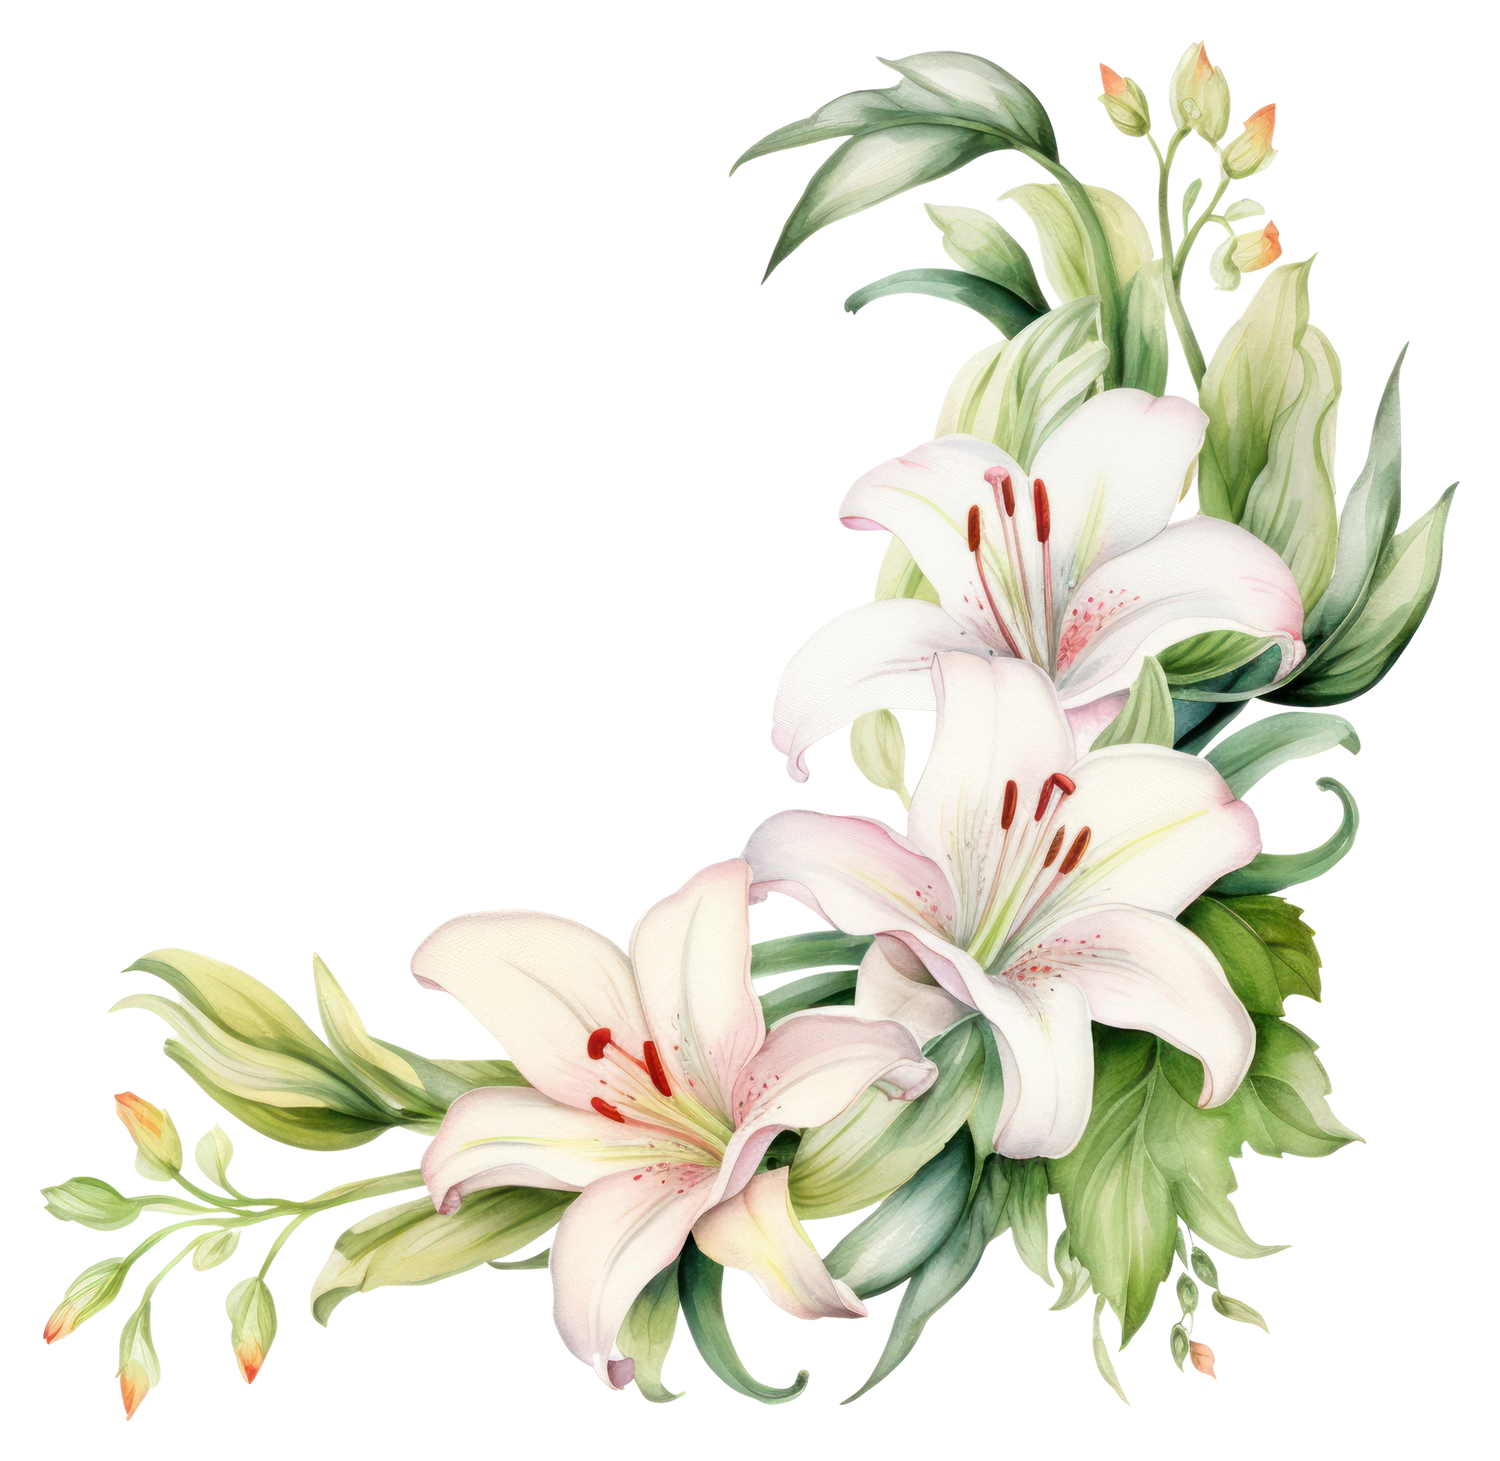
\includegraphics[width=1.3cm]{lily.png}};
  }
}{rmf}

%% 2. AxiomWithDaisy
\newtcbtheorem[no counter]{AxiomWithDaisy}{Axiom}
{%
  enhanced,
  breakable,
  colback = myaxiombg,
  frame hidden,
  boxrule = 0pt,
  borderline west = {2pt}{0pt}{myaxiomfr},
  sharp corners,
  detach title,
  before upper = \tcbtitle\par\smallskip,
  coltitle = myaxiomfr,
  fonttitle = \bfseries\sffamily,
  description font = \mdseries,
  separator sign none,
  segmentation style={solid, myaxiomfr},
  overlay unbroken and last={
    \node[anchor=south east,xshift=-2mm,yshift= -2 mm] at (frame.south east)
      {\includegraphics[width=1.1 cm]{daisy.png}};
  }
}{axd}

%% 3. FactWithOrchid
\newtcbtheorem[no counter]{FactWithOrchid}{Fact}
{%
  enhanced,
  breakable,
  colback = myfactbg,
  frame hidden,
  boxrule = 0pt,
  borderline west = {2pt}{0pt}{myfactfr},
  sharp corners,
  detach title,
  before upper = \tcbtitle\par\smallskip,
  coltitle = myfactfr,
  fonttitle = \bfseries\sffamily,
  description font = \mdseries,
  separator sign none,
  segmentation style={solid, myfactfr},
  overlay unbroken and last={
    \node[anchor=south east,xshift=-2mm,yshift= 0 mm] at (frame.south east)
      {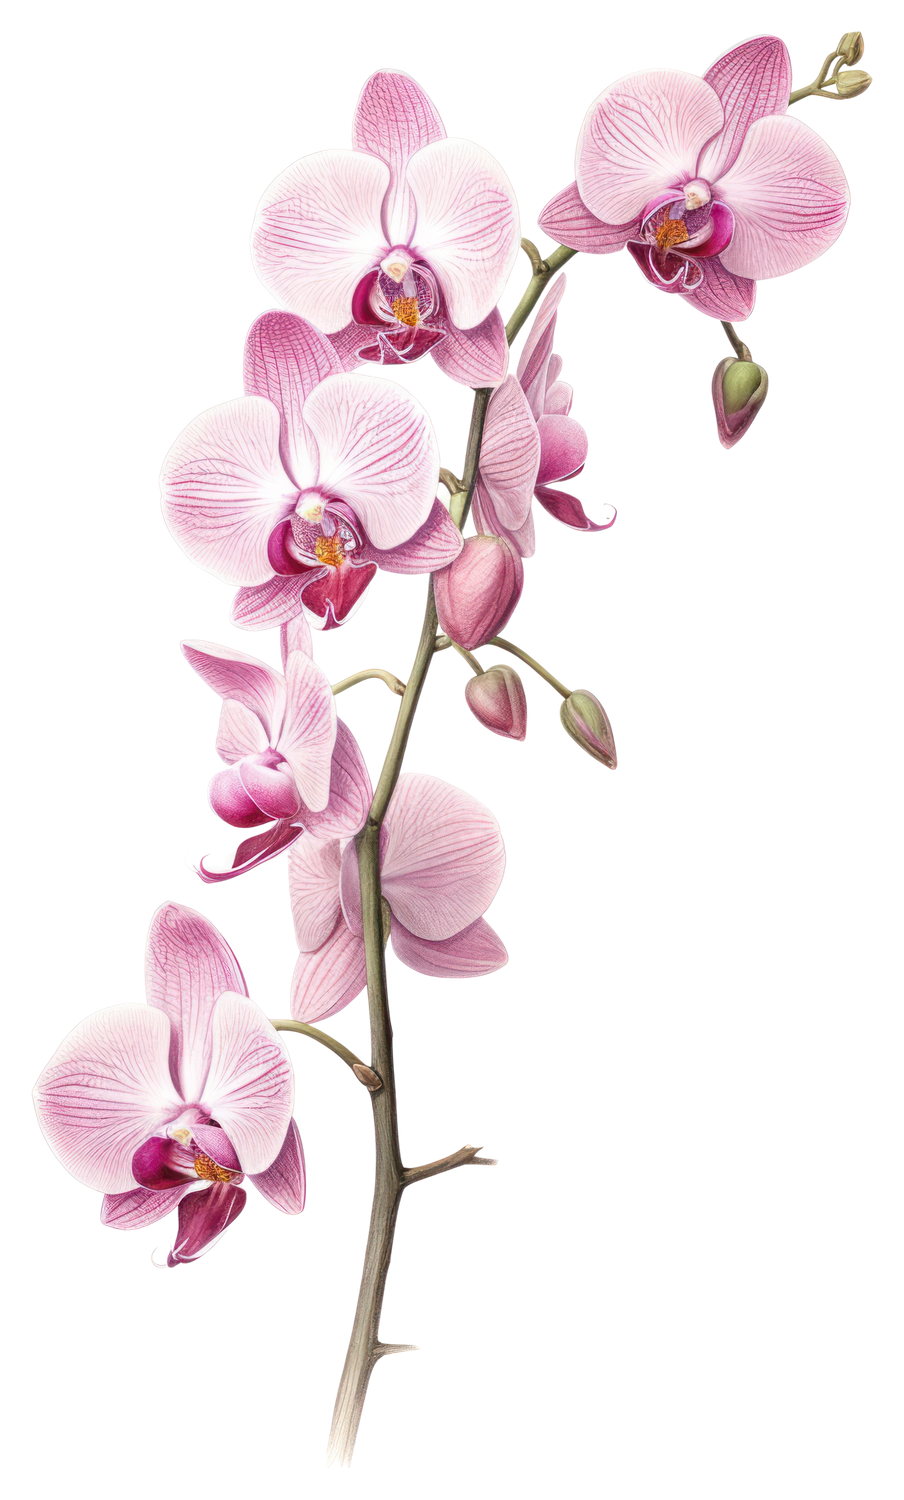
\includegraphics[width= 0.75 cm]{orchid.png}};
  }
}{fco}

%% 4. ConjectureWithSunflower
\newtcbtheorem[no counter]{ConjectureWithSunflower}{Conjecture}
{%
  enhanced,
  breakable,
  colback = myconjbg,
  frame hidden,
  boxrule = 0pt,
  borderline west = {2pt}{0pt}{myconjfr},
  sharp corners,
  detach title,
  before upper = \tcbtitle\par\smallskip,
  coltitle = myconjfr,
  fonttitle = \bfseries\sffamily,
  description font = \mdseries,
  separator sign none,
  segmentation style={solid, myconjfr},
  overlay unbroken and last={
    \node[anchor=south east,xshift=-2mm,yshift=- 1mm] at (frame.south east)
      {\includegraphics[width=1.0 cm]{sunflower.png}};
  }
}{cjsf}

%% 5. ObservationWithCherry
\newtcbtheorem[no counter]{ObservationWithCherry}{Observation}
{%
  enhanced,
  breakable,
  colback = myobsbg,
  frame hidden,
  boxrule = 0pt,
  borderline west = {2pt}{0pt}{myobsfr},
  sharp corners,
  detach title,
  before upper = \tcbtitle\par\smallskip,
  coltitle = myobsfr,
  fonttitle = \bfseries\sffamily,
  description font = \mdseries,
  separator sign none,
  segmentation style={solid, myobsfr},
  overlay unbroken and last={
    \node[anchor=south east,xshift=-2mm,yshift=  0 mm] at (frame.south east)
      {
\includegraphics[width=1.3cm]{cherry.png}};
  }
}{obsch}

%% 6. keyideaWithLotus (already un-numbered)
\newtcolorbox{keyideaWithLotus}{
  enhanced,
  breakable,
  colback = myideabg,
  frame hidden,
  boxrule = 0pt,
  borderline west = {2pt}{0pt}{myideafr},
  sharp corners,
  title = {\bfseries Key Idea},
  detach title,
  before upper = \tcbtitle\par\smallskip,
  coltitle = myideafr,
  overlay unbroken and last={
    \node[anchor=south east,xshift= -1 mm,yshift= 0 mm] at (frame.south east)
      {
\includegraphics[width= 1.3 cm]{lot.png}};
  }
}

%% 7. proofsketchWithHibiscus (already un-numbered)
\newtcolorbox{proofsketchWithHibiscus}{
  enhanced,
  breakable,
  colback = myoutlinebg,
  frame hidden,
  boxrule = 0pt,
  borderline west = {2pt}{0pt}{myoutlinefr},
  sharp corners,
  title = {\bfseries Proof Sketch},
  detach title,
  before upper = \tcbtitle\par\smallskip,
  coltitle = myoutlinefr,
  overlay unbroken and last={
    \node[anchor=south east,xshift=-2mm,yshift=2mm] at (frame.south east)
      {\includegraphics[width=1.1 cm]{hibiscus.png}};
  }
}

%% 8. basecaseWithPoppy (already un-numbered)
\newtcolorbox{basecaseWithPoppy}{
  enhanced,
  breakable,
  colback = mybasebg,
  frame hidden,
  boxrule = 0pt,
  borderline west = {2pt}{0pt}{mybasefr},
  sharp corners,
  title = {\bfseries Base Case},
  detach title,
  before upper = \tcbtitle\par\smallskip,
  coltitle = mybasefr,
  overlay unbroken and last={
    \node[anchor=south east,xshift=-2mm,yshift=-2mm] at (frame.south east)
      {
\includegraphics[width=1.0 cm]{poppy.png}};
  }
}

%% 9. inductstepWithTulip (already un-numbered)
\newtcolorbox{inductstepWithTulip}{
  enhanced,
  breakable,
  colback = mybasebg,
  frame hidden,
  boxrule = 0pt,
  borderline west = {2pt}{0pt}{mybasefr},
  sharp corners,
  title = {\bfseries Inductive Step},
  detach title,
  before upper = \tcbtitle\par\smallskip,
  coltitle = mybasefr,
  overlay unbroken and last={
    \node[anchor=south east,xshift=-2mm,yshift=2mm] at (frame.south east)
      {\includegraphics[width=1.3cm]{tulip.png}};
  }
}

%%%%%%%%%%%%%%%%%%%%%%%%%%%%%%%%%%%%%%%%%%%%%%%%%%%%%%%%%%%%%%%%%%%%%%%%%%%%%
%%  END OF "BIG" PREAMBLE
%%%%%%%%%%%%%%%%%%%%%%%%%%%%%%%%%%%%%%%%%%%%%%%%%%%%%%%%%%%%%%%%%%%%%%%%%%%%%

